% !Rnw weave = Sweave

\documentclass{article}
\title{On the Relationship between Automobile Features and Fuel Efficiency}
\author{D.K. McKinney}
\date{\today}

\usepackage[top=1in, bottom=1in, left=1in, right=1in]{geometry}
\usepackage{verbatim}

\usepackage{Sweave}
\begin{document}
\Sconcordance{concordance:project-RM.tex:project-RM.Rnw:%
1 10 1 1 0 6 1 1 24 1 14 7 1 1 3 11 0 1 2 19 1 1 9 17 0 1 2 10 1 1 10 5 1 1 3 5 %
0 1 2 2 1 1 8 9 1 1 11 13 0 1 2 8 1 1 7 2 1 1 3 10 0 1 2 6 1 1 14 2 1 1 3 11 0 1 %
2 10 1 1 5 8 0 1 2 12 1 1 4 1 2 4 1 1 14 1 2 7 1 1 5 1 2 24 1}

\maketitle


\abstract{The purpose of this research is to identify any fuel efficiencies as measured by vehicle miles driven per gallon of fuel, based upon which of the two most common transmission types automatic and manual. The first phase of the project involves a screening of the data where I identify the extent of missing, inconsistent or anomalous values. The next phase was the preparation of visualization plots. The next phase was the creation of regression models to increase my understanding of the relationships between the different attributes. The final phase involved plotting residuals and performing model diagnostics and other post-hoc testing. 




\section*{Executive Summary}

The final regression model captured 89.46 percent of the total variance and 87.9 percent of the adjusted variance. The coefficents indicate that when the weight of the vehicle increases by 1,000 lbs, the mpg decreases by 3.176 for cars with automatic transmissions, and decreases by 6.099 for cars with manual transmissions. When the quarter-mile performance time increases by 1 second, the mpg increases 0.834 for cars with automatic transmissions and 1.446 for cars with manual transmissions. The answer to the question of whether an automatic or manual transmission is better for MPG would depend on the particular vehicle. The heavier the vehicle, the greater the MPG penalty for having a manual transmission. The quicker the vehicle, the greater the MPG advantage for the manual transmission. The conclusion of this analysis in one sentence is that the MPG variable is largely influenced by the interaction between weight, acceleration and transmission type. T-Testing indicated that the mean difference in MPG between the two transmission types is 7.245 

\begin{center}
\begin{minipage}{0.70\textwidth} 
% latex table generated in R 3.1.0 by xtable 1.7-3 package
% Sat Aug 16 15:57:45 2014
\begin{tabular}{rrrrr}
  \hline
 & Estimate & Std. Error & t value & Pr($>$$|$t$|$) \\ 
  \hline
[Intercept] & 13.9692 & 5.7756 & 2.42 & 0.0226 \\ 
  Automatic:Weight & -3.1759 & 0.6362 & -4.99 & 0.0000 \\ 
  Manual:Weight & -6.0992 & 0.9685 & -6.30 & 0.0000 \\ 
  Automatic:Quarter\_Mile\_Time & 0.8338 & 0.2602 & 3.20 & 0.0035 \\ 
  Manual:Quarter\_Mile\_Time & 1.4464 & 0.2692 & 5.37 & 0.0000 \\ 
   \hline
\end{tabular}

Table 1: Ordinary Least-Squares regression output predicting MPG from the interaction of transmission type, vehicle weight and quarter-mile time.
\end{minipage}
\end{center}


\section*{Introduction}

This analysis is conducted at the behest of Motor Trend Magazine. Motor Trend is particularly interested in exploring the relationships between miles per gallon and the other feature attributes. Two primary points of interest are:

\begin{itemize}
\item Is an automatic or manual transmission better for MPG?
\item What is the MPG difference between automatic and manual transmissions?
\end{itemize}

This analysis will use the mtcars data set to answer their questions using regression models and exploratory data analyses.

\begin{center}
\begin{minipage}{0.55\textwidth} 
% latex table generated in R 3.1.0 by xtable 1.7-3 package
% Sat Aug 16 15:57:45 2014
\begin{tabular}{ll}
  \hline
Name & Description \\ 
  \hline
mpg & Miles/(US) gallon \\ 
  cyl & Number of cylinders \\ 
  disp & Displacement (cu.in.) \\ 
  hp & Gross horsepower \\ 
  drat & Rear axle ratio \\ 
  wt & Weight (lb/1000) \\ 
  qsec & 1/4 mile time \\ 
  vs & Engine Type (0 = V config., 1 = straight config.) \\ 
  am & Transmission (0 = automatic, 1 = manual) \\ 
  gear & Number of forward gears \\ 
  carb & Number of carburetors \\ 
   \hline
\end{tabular}

Table 2: List of variable names and descriptions.

\end{minipage}
\end{center}


\section*{Analysis}

\subsection{Data Processing and Transformations}


The first step in this analysis was to load the data set and view the summary statistics. The data is very clean and has no missing values. The cyl, vs, and am attributes were converted to categorial, or factor variables. The magnitude of hp is much higher than the other attributes so it was normalized. The disp attribute will not be normalized because it is highly correlated with cyl and will be dropped from the analysis. The correlation of each attribute with mpg is:

\begin{center}
\begin{minipage}{0.75\textwidth} 
\begin{Schunk}
\begin{Soutput}
        cyl    disp      hp   drat      wt   qsec    vs     am   gear    carb
mpg -0.8522 -0.8476 -0.7762 0.6812 -0.8677 0.4187 0.664 0.5998 0.4803 -0.5509
\end{Soutput}
\end{Schunk}
\end{minipage}
\end{center}


The next step was to explore MPG graphically in isolation, and by relevant groups. These plots are located at section 5 of the analysis section.


\subsection{T Testing}

The next step was to test the null hypothesis that the MPG fuel efficiency is identical for automatic and manual transmission vechicles. I used the Welch test which assumes unequal variance because it is more conservative with respect to rejecting the null hypothesis. The test provided evidence to reject the null hypothesis of equal MPG for both transmission types.

\begin{center}
\begin{minipage}{0.65\textwidth} 
\begin{Schunk}
\begin{Soutput}
	Welch Two Sample t-test

data:  automatic and manual
t = -3.767, df = 18.33, p-value = 0.001374
alternative hypothesis: true difference in means is not equal to 0
95 percent confidence interval:
 -11.28  -3.21
sample estimates:
mean of x mean of y 
    17.15     24.39 
\end{Soutput}
\end{Schunk}


Table 3: T-test of the hypothesis that there is no MPG difference between types of transmissions.
\end{minipage}
\end{center}


\subsection{Regression Analysis}
My regression strategy was to begin with all attributes, then keep removing the non-factor attribute with the highest p-value until the adjusted R-squared value drops, or no removable attributes remain. I will then compare my best model with an auto-generated model. The best performing model using this strategy uses Transmission Type, Weight, and Horsepower as predictors. Transmission type is not statistically significant but weight and horsepower are.

\begin{center}
\begin{minipage}{0.5\textwidth} 
% latex table generated in R 3.1.0 by xtable 1.7-3 package
% Sat Aug 16 15:57:45 2014
\begin{tabular}{rrrrr}
  \hline
 & Estimate & Std. Error & t value & Pr($>$$|$t$|$) \\ 
  \hline
[Intercept] & 28.5052 & 3.3713 & 8.46 & 0.0000 \\ 
  Manual & 2.0837 & 1.3764 & 1.51 & 0.1413 \\ 
  Weight & -2.8786 & 0.9050 & -3.18 & 0.0036 \\ 
  Horsepower & -2.5696 & 0.6586 & -3.90 & 0.0005 \\ 
   \hline
\end{tabular}
Table 4: Preliminary regression model showing transmission type not significant.
\end{minipage} 
\end{center}

The best model created using a stepwise algorithm uses Weight and Quarter-Mile Time conditioned on Transmission Type.


\begin{center}
\begin{minipage}{0.65\textwidth} 
% latex table generated in R 3.1.0 by xtable 1.7-3 package
% Sat Aug 16 15:57:45 2014
\begin{tabular}{rrrrr}
  \hline
 & Estimate & Std. Error & t value & Pr($>$$|$t$|$) \\ 
  \hline
[Intercept] & 13.9692 & 5.7756 & 2.42 & 0.0226 \\ 
  Automatic:Weight & -3.1759 & 0.6362 & -4.99 & 0.0000 \\ 
  Manual:Weight & -6.0992 & 0.9685 & -6.30 & 0.0000 \\ 
  Automatic:Quarter\_Mile\_Time & 0.8338 & 0.2602 & 3.20 & 0.0035 \\ 
  Manual:Quarter\_Mile\_Time & 1.4464 & 0.2692 & 5.37 & 0.0000 \\ 
   \hline
\end{tabular}
Table 5: Refined model showing interactions are significant among the three attributes.
\end{minipage} 
\end{center}


\subsection{ANOVA}
I will run an ANOVA to compare the two competing models to see if they are significantly different.

\begin{center}
\begin{minipage}{0.5\textwidth} 
% latex table generated in R 3.1.0 by xtable 1.7-3 package
% Sat Aug 16 15:57:45 2014
\begin{tabular}{lrrrrrr}
  \hline
 & Res.Df & RSS & Df & Sum of Sq & F & Pr($>$F) \\ 
  \hline
1 & 28 & 180.29 &  &  &  &  \\ 
  2 & 27 & 118.70 & 1 & 61.59 & 14.01 & 0.0009 \\ 
   \hline
\end{tabular}
Table 6: ANOVA of model comparision.
\end{minipage}
\end{center}


With a p-value of 9e-04 , I reject the null hypothesis which states that the stepwise multivariate model is not significantly different from my hand-rolled model. This is the superior model. 

Before I report the details of this model, it is important to check the residuals for any signs of non-normality and examine the residuals vs. fitted values plot to look for any signs of heteroskedasticity. These diagnostics are located in section 6 of this analysis.


\subsection{Exploratory Plots}

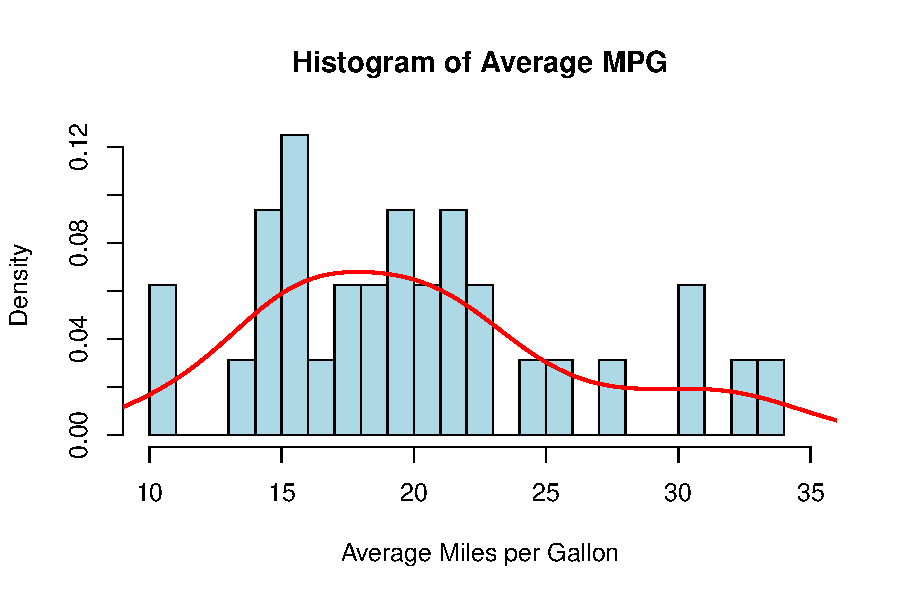
\includegraphics{project-RM-014}

\begin{center}
Plot 1: The histogram of average MPG for the entire sample is multi-modal indicating that the sample is drawn from at least two seperate distributions.
\end{center}

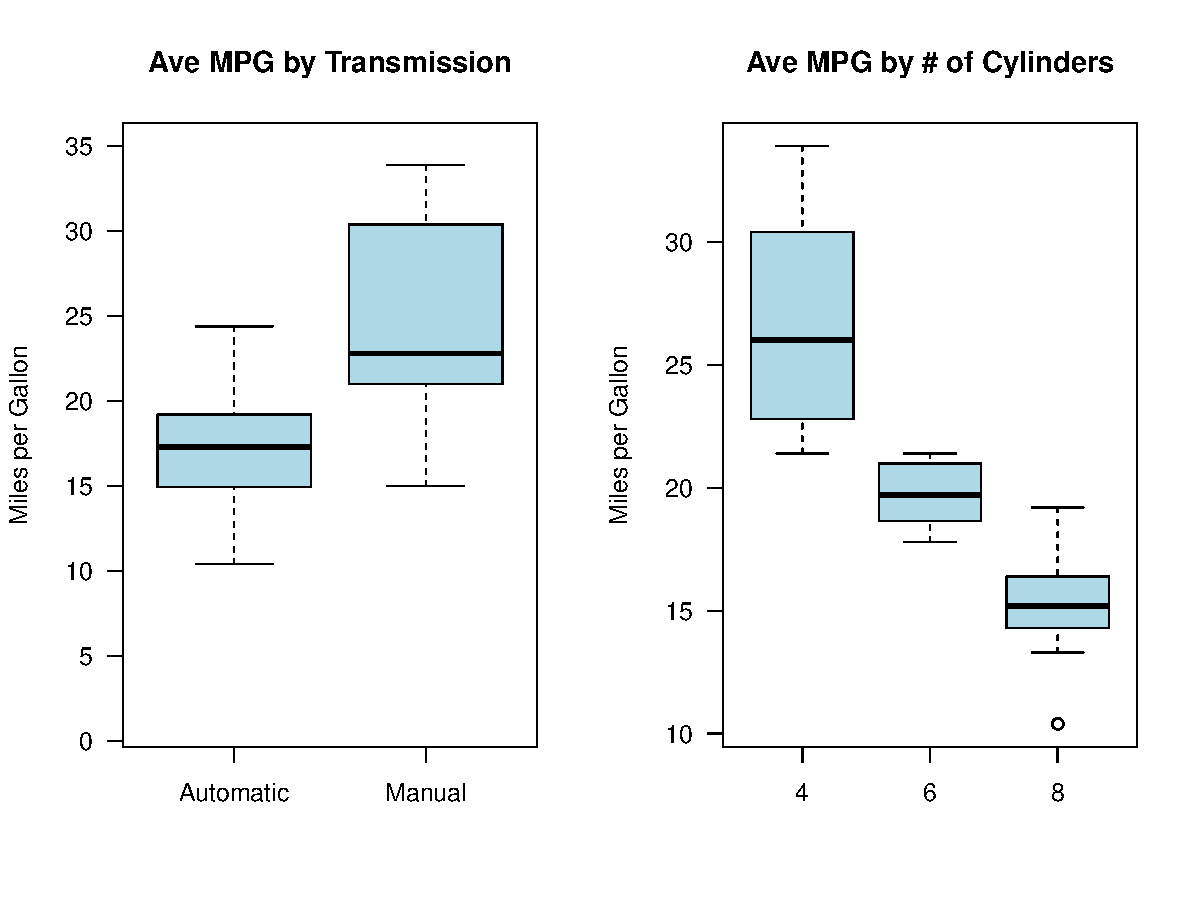
\includegraphics{project-RM-015}

\begin{center}
Plot 2: The histogram of average MPG by transmission type (left) and number of cylinders (right). The group means do not appear to be equal.
\end{center}


\subsection{Residual Plots and Diagnostics}
\begin{center}
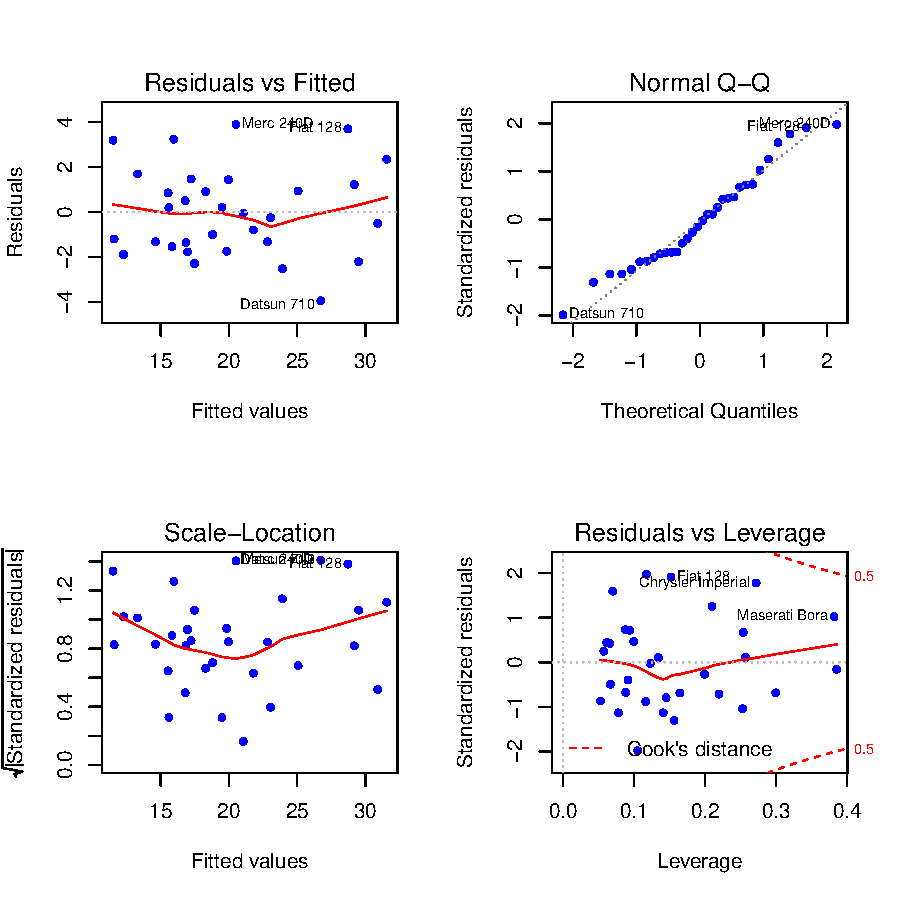
\includegraphics{project-RM-016}
\end{center}

\section*{Conclusion}

The final model captures 89.46 percent of the total variance and
87.9 percent of the adjusted variance. The coefficents
indicate that when the weight of the vehicle increases by 1,000 lbs, the mpg decreases 
by 3.176 for cars with automatic transmissions, and decreases 
by 6.099 for cars with manual transmissions. When the quarter-mile 
performance time increases by 1 second, the mpg increases 0.834 for cars 
with automatic transmissions and 1.446 for cars with manual transmissions. 
This implies that if the car has slower acceleration speeds, other things held constant, cars 
with manual transmissions have larger mpg values. The conclusion of this analysis in one 
sentence is that the mpg variable is largely determined by the relationship between weight 
and accelaration in combination with transmission type.

\begin{thebibliography}{9} 
\bibitem{Jose} Ren{\'{e}} A. Carmona, 
  \emph{Statistical Analysis of Financial Data in S-PLUS}, Springer, 2004. 
\bibitem{LeischI}
Friedrich Leisch. Sweave, part I: Mixing R and Latex. R News, 2(3):28-31, December 2002.
\end{thebibliography}


\end{document}
